\fullscreenimage{Comparing Selection Performance}{roc_explanation}
\fullscreenimage{Current Selection Method Performance}{rocs/rocs_initial}

\displayonelarge{Baseline BDT}{
    As a baseline, train BDT with same inputs as current algorithm. It should perform at least as well.
}{rocs/rocs_bdt1}

\fullscreenimage{Adding Fox-Wolfram Moments to BDT}{fwMoment_ordering}
\displayfour{Fox-Wolfram Distributions}
{fw_moments/fox-wolfram_1}
{fw_moments/fox-wolfram_2}
{fw_moments/fox-wolfram_3}
{fw_moments/fox-wolfram_4}


\displaytwo{BDT with Fox-Wolfram Moments}{
    Improvent from first seven FW Moments is minor, but noticeable.
}{rocs/rocs_bdt2}{rocs/rocs_bdt2_zoom}


\frame{
    \frametitle{Exploring Multi-Jet Discriminants: Centrality}
    \begin{columns}
        \begin{column}{0.5\textwidth}
            {\small The VBF initial scatter quark jets are not always the only thing present in VBF events.
            Radiated Jets (ISR \& FSR) are not uncommon, and provide additional handles for analysis.}
            \begin{figure}
                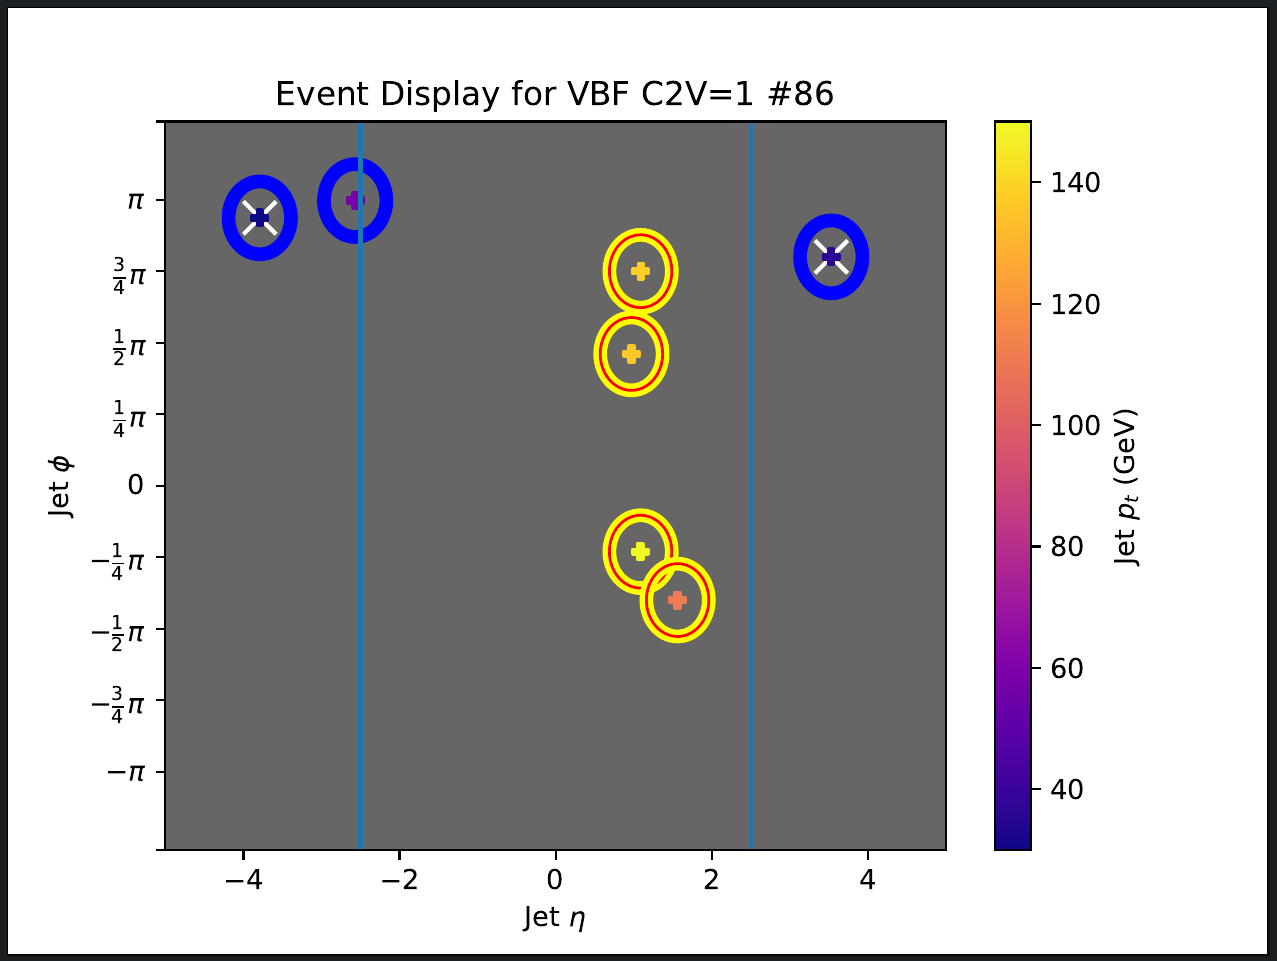
\includegraphics[width=\linewidth,height=\textheight,keepaspectratio]{ event_display}
            \end{figure}
        \end{column}
        \begin{column}{0.5\textwidth}
            \begin{center}\resizebox{0.40\textheight}{!}{ \begin{tikzpicture} \begin{feynman}
    \vertex (a);
    \vertex [right=of a] (b) {H};
    \vertex [above left=of a] (vb1);
    \vertex [below left=of a] (vb2);
    \vertex [left=of vb1] (q1i) {q};
    \vertex [below left=of vb2] (q2k);
    \vertex [left=of q2k] (q2i) {q};
    \vertex [above =of b] (q1f) {q};
    \vertex [below =of b] (q2f) {q};
    \vertex [below =of q2f] (g) {g (ISR)};

    \diagram* {
        (q1i) -- (vb1) -- (q1f),
        (q2i) -- (q2k) -- (vb2) -- (q2f),
        (q2k) --[gluon] (g),
        (vb1) -- [boson] (a) -- [boson] (vb2),
        (a) -- [scalar] (b),
    };
\end{feynman} \end{tikzpicture}
 }\end{center}
            \begin{center}\resizebox{0.40\textheight}{!}{ \begin{tikzpicture} \begin{feynman}
    \vertex (a);
    \vertex [right=of a] (b) {H};
    \vertex [above left=of a] (vb1);
    \vertex [below left=of a] (vb2);
    \vertex [left=of vb1] (q1i) {q};
    \vertex [left=of vb2] (q2i) {q};
    \vertex [below right=of vb2] (q2k);
    \vertex [above =of b] (q1f) {q};
    \vertex [below =of b] (q2f) {q};
    \vertex [below =of q2f] (g) {g (FSR)};

    \diagram* {
        (q1i) -- (vb1) -- (q1f),
        (q2i) -- (vb2) -- (q2k) -- (q2f), 
        (q2k) --[gluon] (g),
        (vb1) -- [boson] (a) -- [boson] (vb2),
        (a) -- [scalar] (b),
    };
\end{feynman} \end{tikzpicture}
 }\end{center}
        \end{column}
    \end{columns}
}


\fullscreenimage{Centrality Distribution}{centrality}
\displaytwo{Centrality as a BDT Input}{
    Improvement from Centrality is very small,
    but there may be more to be gained with further study.
}{rocs/rocs_centrality}{rocs/rocs_centrality_zoom0}
